\documentclass[a4paper]{article}

\usepackage[margin=2.5cm,headheight=50pt,includeheadfoot]{geometry}

\usepackage{amsfonts}
\usepackage{amsmath}
\usepackage{graphicx}
\usepackage{fancyhdr}
\pagestyle{fancy}
\renewcommand{\headrulewidth}{2pt}

\usepackage{xcolor}

\rhead{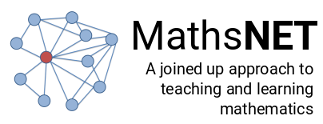
\includegraphics[width=5cm]{../../html/assets/img/logo.png}}
\lhead{\Huge SOR3012: Tutorial week 8}

\begin{document}

\section{Aim}

The aim of the tutorial this week is to look at some more difficult problems on Markov chains in discrete time.

\section{Bring}

Please bring all your notes for this module as well as appropriate items of stationery.

\section{Approach}

You will work in groups of four.  Each group will try to work through as many of the problems below that they can for the first 20 minutes of the tutorial.  During the last 20 minutes of the tutorial 
each group will then be asked to give a two minute presentation of the solution to one of the problems using the visualizer.  You will be told at the start of the tutorial what problem you are 
presenting.  Remember, as you are presenting you should try to write out your solution neatly so that the other students can read what you have done.

\subsection{Question 1}

A Markov chain is described by the following transition matrix:
$$
 \left(
 \begin{matrix}
  1 - 4p & 4p & 0 \\
  2p & 1 - 4p & 2p \\
  0 & 2p & 1 - 2p
 \end{matrix}
 \right)
$$
Determine the range of values which $p$ is allowed to take and the
range of values of $p$ for which the matrix has a limiting stationary
distribution.  Then find the limiting stationary distribution for this
chain.

\subsection{Question 2}

Consider the  reversible  Markov chain, between the
states $X=0,1,2,3,4,5,6,7,8$,  represented  by  the following matrix.
$$
P=
\left(
\begin{matrix}
 0 & 1/2 & 0 & 0& 0 & 1/2 & 0 & 0 & 0 \\
 1/3 & 0 & 1/3 & 0 & 1/3 & 0 & 0 & 0 & 0 \\
 0 & 1/2 & 0 & 1/2 & 0 & 0 & 0 & 0 & 0 \\
 0 & 0 & 1/3 & 0 & 1/3 & 0 & 0 & 0 & 1/3\\
 0 & 1/4 & 0 & 1/4 & 0 & 1/4 & 0 & 1/4 & 0\\
 1/3 & 0 & 0 & 0 & 1/3 & 0 &  1/3 & 0 & 0 \\
 0 & 0 & 0 & 0 & 0 & 1/2 & 0 & 1/2 & 0 \\
 0 & 0 & 0 & 0 & 1/3 & 0 & 1/3 & 0 & 1/3\\
 0 & 0 & 0 & 1/2 & 0 & 0 & 0 & 1/2 & 0   \\
\end{matrix}
\right) \qquad .
$$
Draw the transition graph for this process (hint: start by drawing a 3 x 3 grid
of nodes with 0, 5 and 6 on the top row 1,4 and 7 on the second row and 2,3 and
8 on the bottom row).  Then find the stationary distribution by using the detailed
balance condition.

\subsection{Question 3}

A double glazing firm employs staff to cold call clients and try to sell
them new windows for their home. There are three levels of staff pay: Level 1
(\pounds~50), Level 2 (\pounds~75) or Level 3 (\pounds~100).  The amount a
person is paid in a given evening is determined by their performance
that evening and their performance on the previous evening.  A staff member who
was paid at level 1 on the previous day is moved to level 2 if they are
amongst the top 80\% of sellers that evening. Similarly a staff member on level
2 the previous evening is moved to level 3 if they are amongst the top 80\% this evening. Members of staff in the bottom 20% have their pay reduced by
at least one level.  If they are in level 2 their pay falls to that of
level 1.  If they are in level 3 they fall to level 1 if they are in the bottom
5\% and level 2 otherwise. If the company employs
$n$ members of staff, calculate the average amount they would expect to pay out
in salaries each evening.  You may assume that the performance of any given
member of the sales team is random and hence that the ordering of
staff performances is random.

\subsection{Question 4}


A magazine has print and ipad editions and 100,000 subscribers. These
subscribers can subscribe to the magazine in
one of three ways. They can buy the print magazine only, they can buy an ipad
subscription only or they can buy both an ipad and a print subscription to the
magazine.  The magazine is constantly changing its content and there is not
always a complete overlap between the features in the ipad and print versions of
the magazine.  As a consequence people are continuously changing their
subscription package. In any given week no one ever changes from a
purely print subscription to the ipad edition and vice versa.  However, every
week a constant fraction, $p$, of the subscribers on a print only subscription
change to the ipad+print subscription.  Similarly $p$ subscribers on
an ipad only subscription change to the ipad+print subscription every week. Of
those subscribers on the ipad+print subscription a fraction, $2p$, of them
decide which version of the magazine they prefer in any given week and adjust
their subscription accordingly. Subscribers are split 50/50 on which version of
the magazine they prefer so $p$ change to ipad only, while the other $p$
change to print only.  Explain why the level of subscription a person has to
the magazine is a Markov process, draw the transition graph and write down the
transition matrix for the random variable. Calculate the average number of
magazines
that need to be printed each week in order to satisfy the demand for printed
editions.

\subsection{Question 5}

I own 4 umbrellas and keep some in my home and some in my
office.  I keep moving between my home and office and only take one of my
umbrellas with me if it rains.  Obviously, if it does not rain I do not take an
umbrella. The probability of rain on any given day is equal to $p$. Explain
why the number of umbrellas in my current location, $S$, is a Markov process,
draw the transition graph for this variable and write out the transition matrix.
When doing this remember that if there are 3 umbrellas in my office, $S_i=3$,
and it doesn't rain there will be 1 umbrella available for me once I get home,
$S_{i+1}=1$, and set out to the office once more.
Now use the Markov chain you have drawn to solve the following problem:
If I am in my office/home when it rains and there are no
umbrellas available I will get wet as I walk to home/work.  Using the
detailed balance condition or otherwise show that if $p=0.6$ the probability
this will occur is approximately 5.4 \%.  How many umbrellas should I buy if I
want the probability of getting wet to be less than 1 \%.









\end{document}
